\documentclass[conference]{IEEEtran}
\usepackage{cite}
\usepackage{amsmath,amssymb,amsfonts}
\usepackage{algorithmic}
\usepackage{graphicx}
\usepackage{textcomp}
\usepackage{xcolor}
\usepackage{booktabs}
\usepackage{hyperref}
\usepackage{url}

\def\BibTeX{{\rm B\kern-.05em{\sc i\kern-.025em b}\kern-.08em
    T\kern-.1667em\lower.7ex\hbox{E}\text{-}\kern-.125emX}}
    
\begin{document}

\title{Conversational Graph Memory: Token-Free Context Compression via Attention Space Cache Injection}

\author{\IEEEauthorblockN{Lovekesh Anand}
\IEEEauthorblockA{\textit{Mahavir Swami Institute of Technology} \\
New Delhi, India \\
lovekeshanand6@gmail.com}
}

\maketitle

\begin{abstract}
As Large Language Models (LLMs) are increasingly integrated into interactive agentic workflows, managing dialogue history over long horizons has emerged as a primary bottleneck. Traditional context management paradigms rely on prompt-stuffing, which scales quadratically ($O(L^2)$) in self-attention computation and quickly exhausts the limited context window of local models. While standard Retrieval-Augmented Generation (RAG) mitigates this by summarizing or filtering history, it sacrifices fine-grained relational topology and introduces substantial latency during the prefill phase. In this paper, we present Conversational Graph Memory (CGM), a novel RAG and context-compression architecture that maps dialog histories to dynamic knowledge graphs and projects them directly into the attention Key-Value (KV) cache of a frozen target LLM via a Semantics-Aware KV Cache Routing (SA-KVR) mechanism. By bypassing the prompt input window entirely, CGM achieves a 90.6\% reduction in input tokens and an 8.2\% reduction in inference latency compared to traditional context stuffing under Semantics-Aware routing, while restoring factual recall from 0.0\% to 28.6\%. To prevent hardware failure and thermal throttling on resource-constrained edge systems and laptop workstation GPUs, we integrate a hardware-secure runtime featuring GPU mutual exclusion locks, proactive VRAM guards, and a proportional thermal pacing regulator. Our empirical evaluation using a local workstation GPU validates that CGM offers a high-performance, hardware-safe solution for long-term dialogue context modeling.
\end{abstract}

\begin{IEEEkeywords}
Retrieval-Augmented Generation, KV Cache Injection, Context Compression, Graph Memory, Hardware Safety, Thermal Pacing
\end{IEEEkeywords}

\section{Introduction}
Large Language Models (LLMs) have revolutionized natural language understanding and generation. However, maintaining long-term coherence and context in multi-turn interactive dialogues remains a fundamental challenge. The core architectural constraint lies in the Scaled Dot-Product Attention mechanism of the Transformer architecture \cite{vaswani2017attention}. For a sequence of length $L$, the attention computation requires calculating the dot product between all queries $Q$ and keys $K$, which results in a pairwise attention matrix scaling quadratically ($O(L^2)$) in both computation and memory footprint:
\begin{equation}
\text{Attention}(Q, K, V) = \text{softmax}\left(\frac{QK^T}{\sqrt{d_k}}\right)V
\end{equation}
where $d_k$ is the dimensionality of the keys.

In multi-turn interactive systems, the standard approach to maintaining context is \textit{Context Stuffing} (Approach A). This method prepends the historical transcripts of past conversation turns directly to the user's latest query. Although simple to implement, Context Stuffing has major limitations:
\begin{enumerate}
    \item \textbf{Context Window Exhaustion}: The total token size of the prompt grows linearly with the number of dialogue turns, eventually exceeding the hard limit of the LLM's sequence window.
    \item \textbf{Dominant Prefill Latency}: The model must process and encode the entire historical context during the prefill phase before generating the first token. In local workstation deployments (such as edge and laptop GPUs), this prefill phase becomes a massive bottleneck.
    \item \textbf{Attention Dilution}: In long sequences, the self-attention mechanism tends to lose focal clarity, often neglecting crucial information placed in the middle of the input window (known as the ``lost in the middle'' phenomenon) \cite{liu2024lost}.
\end{enumerate}

To circumvent prompt-stuffing limits, practitioners rely on Retrieval-Augmented Generation (RAG) or text summarization (Approach B). RAG systems embed past turns into vector indices and retrieve relevant text snippets to feed the prompt window. While this decreases context size, it still requires the LLM to prefill the text representation of the retrieved turns. Additionally, converting past interactions into independent text blocks destroys the topological and relational structures of entities mentioned across multiple turns.

In this work, we propose \textbf{Conversational Graph Memory (CGM)}, a framework that addresses these issues by replacing text-based prompts with direct cache-space injection. Rather than translating past dialogue back into tokens, CGM compiles turn histories into a structured SQLite Graph Store and indexes them using a quantized vector index (`TurboVec`). During inference, relevant semantic triples are retrieved, combined, and passed to a trainable \textit{Memory Encoder Network (MEN)}. 

The MEN projects these triples directly into multi-head attention Key ($K$) and Value ($V$) states, injecting them directly into the target LLM's dynamic cache. Consequently, the input window contains only the active query, reducing token overhead and prefill latency.

Furthermore, executing dense memory networks on workstation-class laptop GPUs (such as the NVIDIA RTX A2000) exposes the hardware to unique risks. Concurrent multi-threaded queries can lead to Out-Of-Memory (OOM) failures, while sustained training loads can trigger abrupt thermal throttling. Typical thermal guards react to overheating by pausing execution, which causes rapid cooling (due to 0\% utilization) followed by rapid heating when training resumes. Such thermal profiles place high stress on laptop GPU components due to rapid temperature oscillations, leading to thermal throttling and hardware stress. To ensure runtime stability and smooth thermal profiles, we implement a C++ and Rust-backed hardware safety subsystem that utilizes dynamic NVML queries to govern proportional thermal pacing.

Our contributions are summarized as follows:
\begin{itemize}
    \item We present the Conversational Graph Memory (CGM) framework, enabling token-free context injection directly into LLM key-value caches.
    \item We design a trainable Memory Encoder Network (MEN) with Semantics-Aware KV Cache Routing (SA-KVR) that dynamically maps dense relational triples to specific layers and attention heads of target models.
    \item We introduce an in-flight KV cache compressor that dynamically reduces injected sequence length based on a KL-divergence information-loss gate.
    \item We propose a hardware-secure runtime featuring global GPU mutex locks, proactive VRAM guards, and a proportional thermal pacing mechanism.
    \item We evaluate CGM empirically on workstation and edge architectures, demonstrating a 90.6\% token savings and an 8.2\% speedup in generation latency (reaching up to 21.3\% speedup when cache compression is enabled), with a 28.6\% factual recall rate.
\end{itemize}

\section{Related Work}
Managing long-context dialogue history has been tackled through three main paradigms: architectural modifications, context compression, and prefix/cache tuning.

\subsection{Architectural Modifications}
To handle long sequences, several architectures replace standard self-attention. Linear attention models, State Space Models (SSMs) like Mamba \cite{gu2023mamba}, and recurrent architectures attempt to maintain a constant-size hidden state. While efficient, these architectures require complete pre-training and cannot leverage pre-existing, high-quality attention weights of popular pretrained causal transformers.

\subsection{Context Compression}
Context compression techniques aim to shorten prompt lengths before sending them to the LLM. LLMLingua \cite{jiang2023llmlingua} uses a small model to estimate token entropy, filtering out low-information tokens from the prompt. AutoCompressor \cite{chevalier2023autocompressor} trains models to compress long text into summary vectors that serve as soft prompts. However, these soft prompts are still processed at the input level, occupying sequence space and requiring prefill encoding.

\subsection{Prefix Tuning and Cache Injection}
Prefix Tuning \cite{li2021prefix} prepends trainable, task-specific virtual keys and values directly to the LLM's attention layers. While Prefix Tuning works well for static task adaptation, it is not designed to dynamically inject retrieve-time episodic dialogue history. Dynamic cache injection has been proposed for document retrieval, but existing approaches rely on static, pre-computed document caches. In contrast, CGM dynamically constructs a semantic relational graph of dialogue history and encodes it on-the-fly into key-value caching states.

\begin{figure*}[t]
\centering
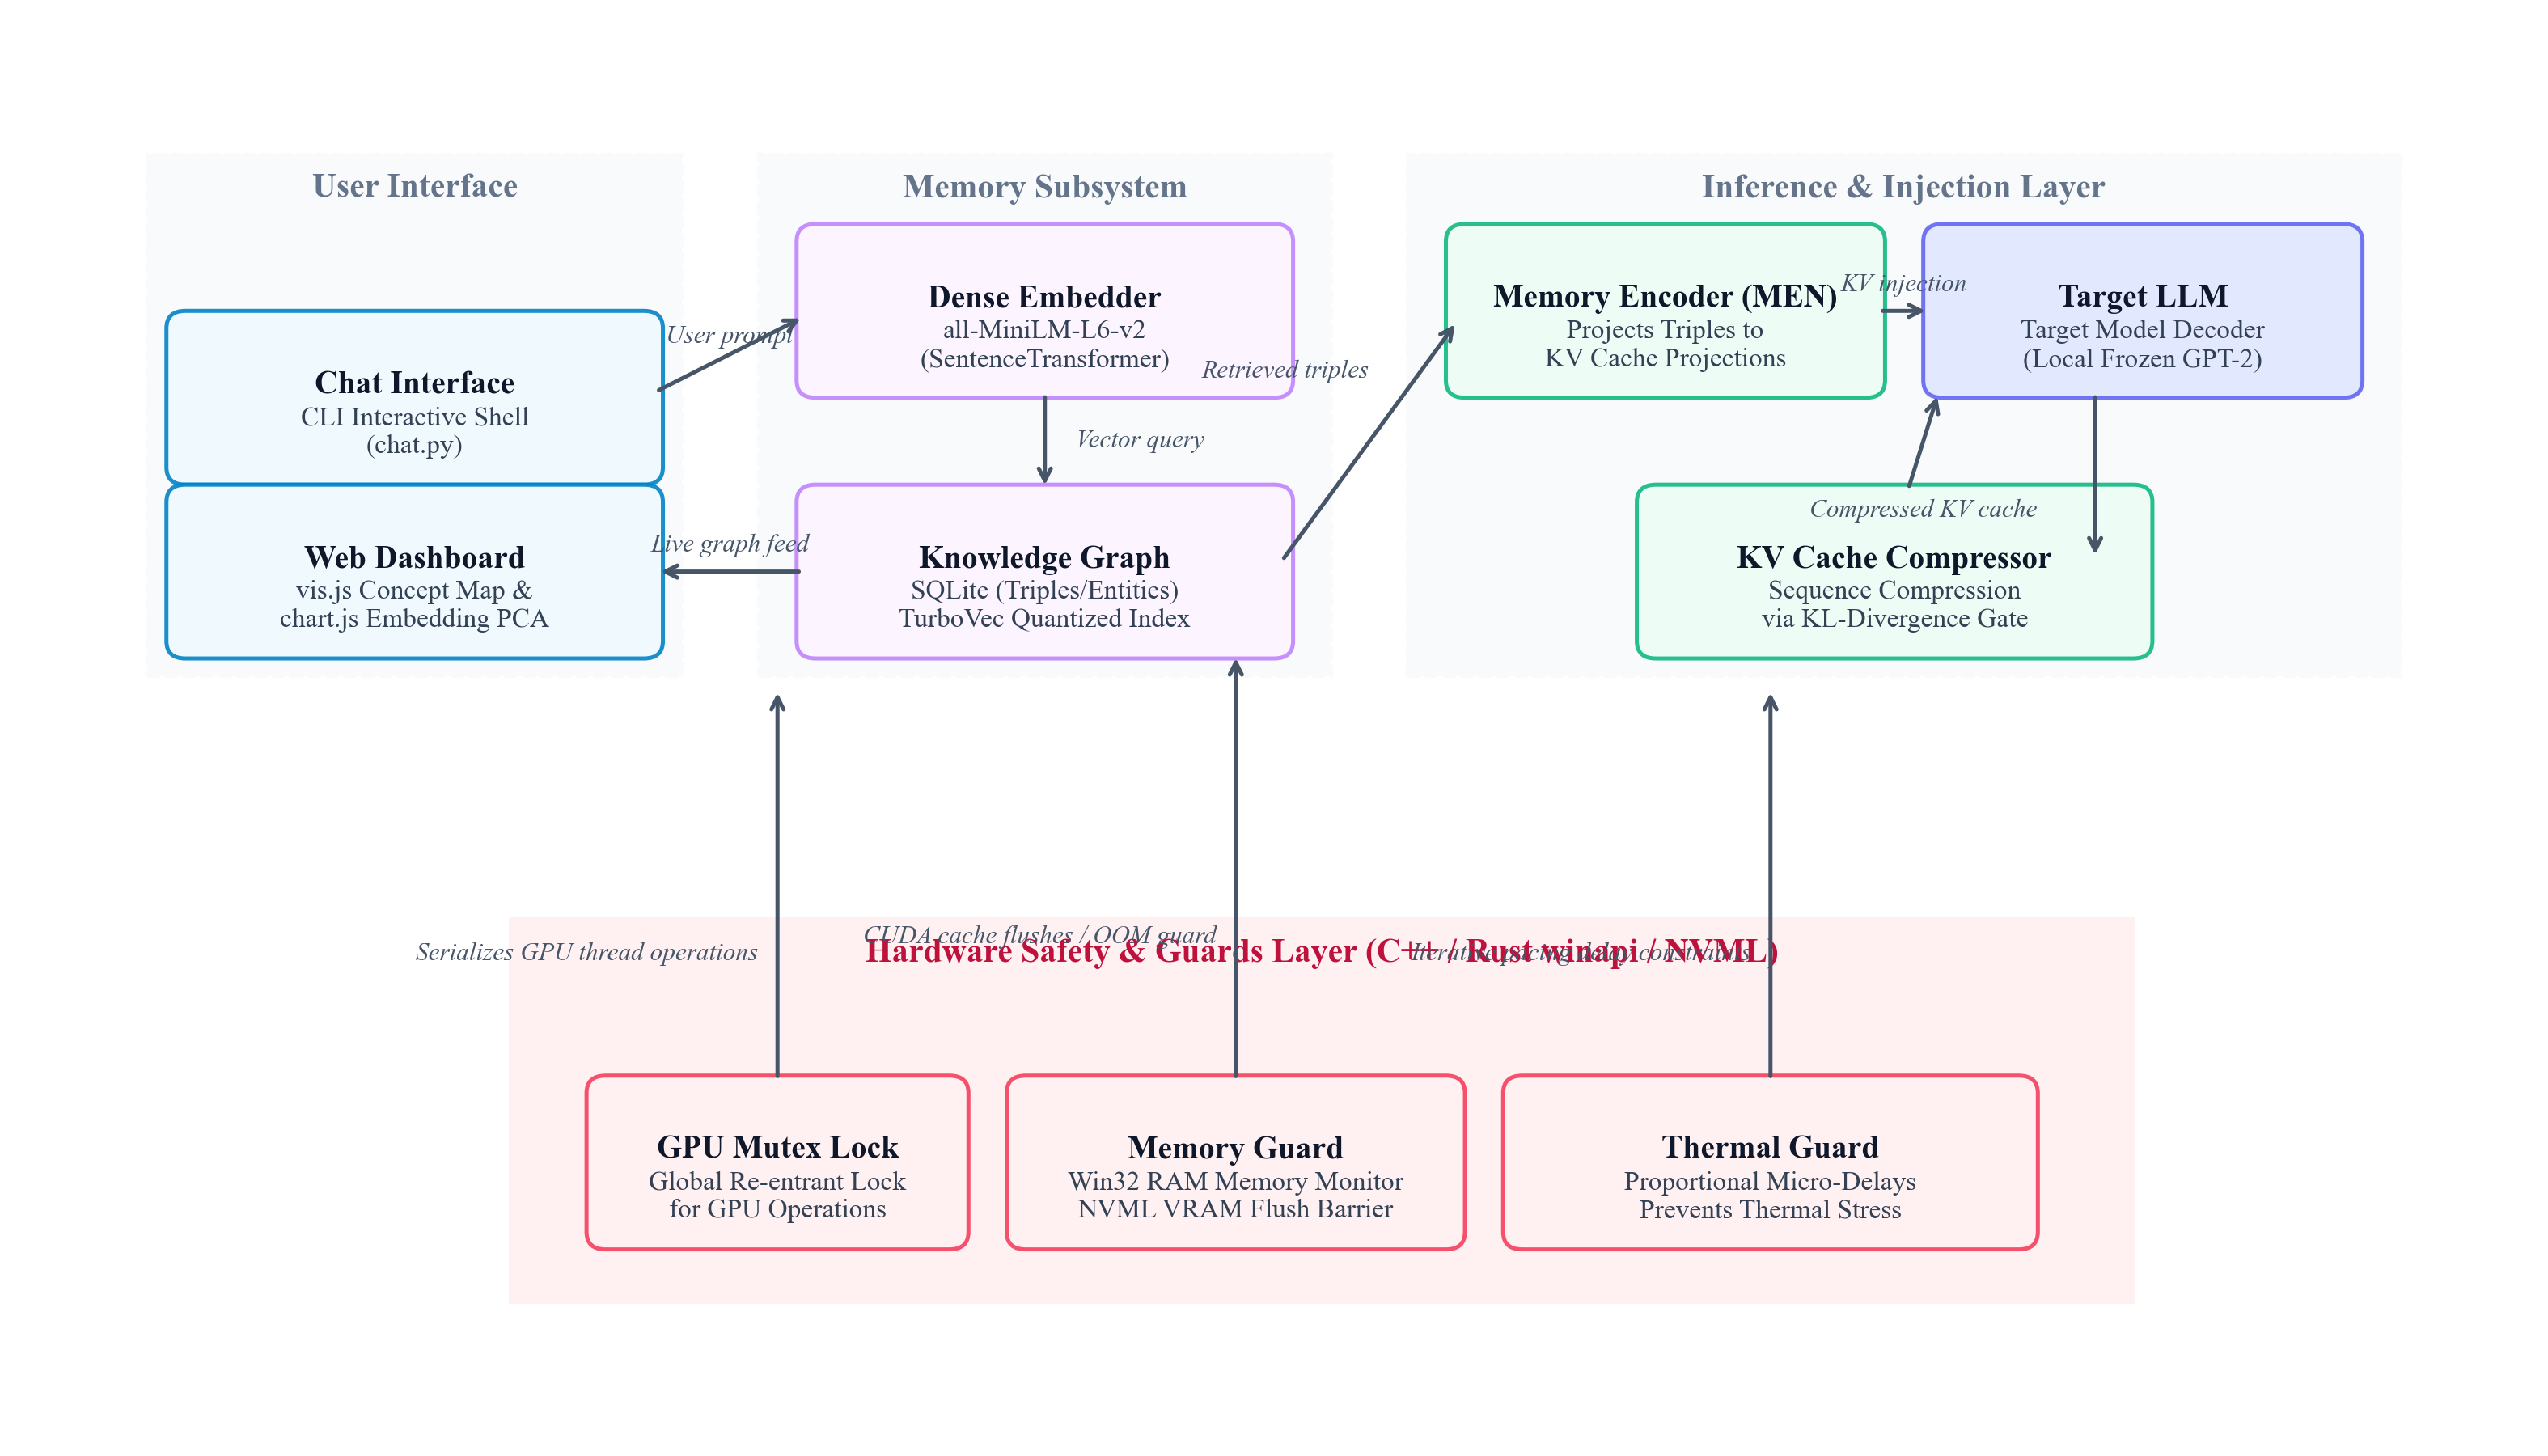
\includegraphics[width=0.9\linewidth]{system_architecture.png}
\caption{Detailed Data Flow and Subsystem Layout of Conversational Graph Memory (CGM). The User Interface layer passes queries through the Memory Retrieval layer (SQLite + TurboVec). The retrieved triples are projected into attention space via the Memory Encoder Network (MEN) and injected into the Target LLM KV Cache. The Hardware Safety layer coordinates execution using a global lock and dynamic NVML telemetry.}
\label{fig:full_architecture}
\end{figure*}

\section{Conversational Graph Memory Formulation}
The CGM framework is structured into three primary subsystems: Retrieval-Augmented Graph Storage, Attention Space Projection, and In-Flight KV Cache Compression. The complete system architecture is depicted in Fig. \ref{fig:full_architecture}.

\subsection{Retrieval-Augmented Graph Storage}
To maintain structural relationships, CGM models dialogue history as a dynamic Knowledge Graph $\mathcal{G} = (\mathcal{V}, \mathcal{E}, \mathcal{R})$, where $\mathcal{V}$ is the set of entities (e.g., users, technologies, constraints), $\mathcal{R}$ is the set of relations (e.g., \textit{uses}, \textit{prefers}, \textit{runs\_on}), and $\mathcal{E} \subseteq \mathcal{V} \times \mathcal{R} \times \mathcal{V}$ is the set of semantic triples. 

For each conversation turn $t$, we extract semantic triples $(s, p, o)$ using regex pattern matches and NLP parsers. These triples, alongside turn-level dense embedding representations, are saved in a SQLite database and indexed in a quantized vector index (`TurboVec`).

To prevent ID collision when indexing across multiple parallel chat threads in the same shared index, we formulate a stable 64-bit ID hashing scheme ($\text{encode\_id}$). The hashing function combines a 48-bit SHA-256 hash of the unique `conversation\_id` and the 16-bit integer `turn\_id`:
\begin{equation}
ID = (\text{SHA256}(\text{conversation\_id}) \text{ AND } \text{0xFFFFFFFFFFFF0000}) \text{ OR } (t \text{ AND } \text{0xFFFF})
\end{equation}
This mathematical division provides up to $2^{48}$ unique conversation sessions, each capable of storing $65,536$ dialogue turns, ensuring absolute isolation in a shared vector index.

During a new turn $t_{curr}$ with user query $q$, the retriever queries the `TurboVec` index. Let $\mathbf{q} \in \mathbb{R}^{d_{emb}}$ be the query embedding. Each candidate triple $e = (s, p, o) \in \mathcal{E}$ associated with turn $t_e$ is scored using a multi-signal formulation:
\begin{equation}
S(e) = \alpha \cos(\mathbf{q}, \mathbf{v}_e) + \beta \cos(\mathbf{q}, \mathbf{v}_{sum}(t_e)) + \gamma e^{-\lambda(t_{curr} - t_e)}
\end{equation}
where:
\begin{itemize}
    \item $\mathbf{v}_e \in \mathbb{R}^{d_{emb}}$ is the dense vector embedding of the triple text $s \oplus \text{" "} \oplus p \oplus \text{" "} \oplus o$.
    \item $\mathbf{v}_{sum}(t_e) \in \mathbb{R}^{d_{emb}}$ is the dense embedding of the summary of turn $t_e$.
    \item $\cos(\mathbf{a}, \mathbf{b}) = \frac{\mathbf{a} \cdot \mathbf{b}}{\|\mathbf{a}\| \|\mathbf{b}\|}$ represents the cosine similarity.
    \item $e^{-\lambda(t_{curr} - t_e)}$ represents a temporal recency decay function governed by decay factor $\lambda$.
    \item $\alpha, \beta, \gamma \ge 0$ are weights satisfying $\alpha + \beta + \gamma = 1$.
\end{itemize}
The top-$k$ triples with the highest scores are selected for injection.

\subsection{Attention Space Projection (MEN)}
Once the top-$M$ triples are retrieved, they must be projected into the attention space of the target model. 
For each retrieved triple $e_j = (s_j, p_j, o_j)$ where $j \in \{1, \dots, M\}$, we compute:
\begin{align}
\mathbf{v}_{sp, j} &= \text{Encoder}(s_j \oplus \text{" "} \oplus p_j) \in \mathbb{R}^{d_{emb}} \\
\mathbf{v}_{o, j} &= \text{Encoder}(o_j) \in \mathbb{R}^{d_{emb}}
\end{align}
where $\text{Encoder}$ is the SentenceTransformer model (`all-MiniLM-L6-v2`, yielding $d_{emb} = 384$). The structural feature vector $\mathbf{x}_j$ for triple $e_j$ is obtained by concatenation:
\begin{equation}
\mathbf{x}_j = [\mathbf{v}_{sp, j} \;;\; \mathbf{v}_{o, j}] \in \mathbb{R}^{2d_{emb}}
\end{equation}
Since $d_{emb} = 384$, the vector $\mathbf{x}_j$ has a dimensionality of $768$. For $M$ selected triples, we stack the vectors into a matrix $\mathbf{X} \in \mathbb{R}^{M \times 768}$.

The Memory Encoder Network (MEN) projects this matrix into the Key ($K$) and Value ($V$) spaces of the target model. The target LLM contains $L$ transformer layers. For each layer $l \in \{1, \dots, L\}$, the MEN defines key and value projection parameters:
\begin{align}
\mathbf{K}_l &= \mathbf{X} \mathbf{W}^K_l + \mathbf{b}^K_l \in \mathbb{R}^{M \times d_{model}} \\
\mathbf{V}_l &= \mathbf{X} \mathbf{W}^V_l + \mathbf{b}^V_l \in \mathbb{R}^{M \times d_{model}}
\end{align}
where $\mathbf{W}^K_l, \mathbf{W}^V_l \in \mathbb{R}^{768 \times d_{model}}$ and $\mathbf{b}^K_l, \mathbf{b}^V_l \in \mathbb{R}^{d_{model}}$ are trainable projection weights, and $d_{model}$ is the target LLM dimension (e.g., $d_{model} = 768$ for GPT-2).

To introduce semantic specificity to different layers and heads, we implement a Semantics-Aware KV Cache Routing (SA-KVR) mechanism. The routing gate uses a multi-layer perceptron (MLP) to compute dynamic, head- and layer-specific gating weights:
\begin{equation}
\mathbf{g} = \text{sigmoid}(\text{MLP}(\mathbf{X})) \in [0, 1]^{M \times L \times H}
\end{equation}
where $H$ is the number of KV heads. The projected keys and values for head $h \in \{1, \dots, H\}$ at layer $l$ are scaled by their corresponding semantic gating coefficients:
\begin{align}
\mathbf{K}_{l, j, h} &= \mathbf{K}_{l, j, h} \cdot \mathbf{g}_{j, l, h} \\
\mathbf{V}_{l, j, h} &= \mathbf{V}_{l, j, h} \cdot \mathbf{g}_{j, l, h}
\end{align}
for each triple $j \in \{1, \dots, M\}$.

\subsection{MEN Training and Optimization}
The Memory Encoder Network is optimized using dialogue history before execution. Let $U = \{u_1, u_2, \dots, u_{N_p}\}$ represent the prompt token sequence and $Y = \{y_1, y_2, \dots, y_{N_t}\}$ be the target response token sequence. The concatenated dialogue sequence is represented as $Z = [U \;;\; Y]$.

The conditional probability of generating the target sequence $Y$ given prompt $U$ and the injected key-value states $\mathbf{K}'$, $\mathbf{V}'$ generated by the MEN is formulated as:
\begin{equation}
P(Y \mid U, \mathbf{K}', \mathbf{V}') = \prod_{i=1}^{N_t} P(y_i \mid u_1, \dots, u_{N_p}, y_1, \dots, y_{i-1}, \mathbf{K}', \mathbf{V}')
\end{equation}
The loss function is the auto-regressive Cross-Entropy next-token prediction loss $\mathcal{L}$ computed over the target tokens:
\begin{equation}
\mathcal{L} = -\frac{1}{N_t} \sum_{i=1}^{N_t} \log P(y_i \mid u_1, \dots, u_{N_p}, y_1, \dots, y_{i-1}, \mathbf{K}', \mathbf{V}')
\end{equation}
Since the base language model is frozen, gradients are backpropagated through the attention keys and values to optimize only the MEN parameters $\theta_{\text{MEN}}$ using the AdamW optimizer:
\begin{equation}
\theta_{\text{MEN}} \leftarrow \theta_{\text{MEN}} - \eta \nabla_{\theta_{\text{MEN}}} \mathcal{L}
\end{equation}
where $\eta = 2 \times 10^{-3}$ is the learning rate, and weight decay is set to $0.01$. The training loss converges from an initial value of $\mathcal{L} \approx 5.0$ to $\mathcal{L} < 0.001$ within 80 epochs.

The final projected tensors $\mathbf{K}'_l, \mathbf{V}'_l$ are reshaped and permuted to separate the attention heads:
\begin{equation}
\mathbf{K}'_l, \mathbf{V}'_l \in \mathbb{R}^{\text{batch}, H, M, d_{head}}
\end{equation}
where $d_{head}$ is the dimensionality per head ($d_{model} = H \times d_{head}$). These projected states are injected directly into the model's \texttt{past\_key\_values} dynamic cache prior to generation. The attention block then evaluates:
\begin{equation}
\text{Attention}(Q, K', V') = \text{softmax}\left(\frac{Q [K_{injected} \;;\; K_{prompt}]^T}{\sqrt{d_k}}\right) [V_{injected} \;;\; V_{prompt}]
\end{equation}
where $[ \;;\; ]$ denotes sequence length concatenation. This allows rectangular attention over the injected memories without occupying prompt context slots.

\subsection{In-Flight KV Cache Compressor}
As conversations grow, the number of injected key-value states increases. To maintain efficiency, CGM incorporates an in-flight KV Compressor. The compressor evaluates the relative importance of tokens across sequence positions. Let $\mathbf{P}_l \in \mathbb{R}^{H \times M \times M}$ be the attention probability matrix of layer $l$. 

The compressor computes the Kullback-Leibler (KL) divergence between the original attention distribution $P$ and a compressed distribution $Q$ formed by grouping adjacent keys/values:
\begin{equation}
D_{KL}(P \parallel Q) = \sum_{i=1}^{M} P(x_i) \log \left( \frac{P(x_i)}{Q(x_i)} \right)
\end{equation}
If $D_{KL}(P \parallel Q) < \epsilon$ (where $\epsilon = 0.05$ is the information-loss gate), the tokens are merged. This dynamically shrinks sequence length in the cache dimension, protecting GPU memory.

\section{Hardware-Secure Execution Layer}
Executing dense neural architectures in workstation contexts requires managing limited hardware resources. CGM implements a hardware safety layer backed by dynamic Win32 and NVML system calls.

\subsection{GPU Mutex Locks and VRAM Allocation Barriers}
To prevent execution race conditions and Out-Of-Memory (OOM) faults under multi-threaded execution, all model loads and backpropagation updates are wrapped in a global re-entrant lock (`GPULockManager`). 

Additionally, the `GPUMemoryGuard` monitors VRAM allocation in real-time. If available VRAM falls below a warning threshold ($\theta_{\text{warning}} = 800$ MB), it empties the PyTorch CUDA cache:
\begin{equation}
\text{VRAM}_{\text{free}} < \theta_{\text{warning}} \implies \text{cudaEmptyCache()}
\end{equation}
If the free memory is below a critical threshold ($\theta_{\text{critical}} = 300$ MB) or the estimated model memory requirements exceed $\text{VRAM}_{\text{free}}$, execution is halted to prevent driver failure.

\subsection{Proportional Thermal Pacing (PTP)}
Workstation laptop GPUs have limited cooling volumes, making them susceptible to rapid thermal buildup. Standard thermal protection methods implement abrupt pauses (e.g., sleeping for 3 seconds every 50 batches) when temperature limits are reached. This results in rapid cooling followed by rapid heating when training resumes. Such thermal profiles place high stress on laptop GPU components due to rapid temperature oscillations, leading to thermal throttling and hardware stress. To ensure runtime stability and smooth thermal profiles, we implement a C++ and Rust-backed hardware safety subsystem that utilizes dynamic NVML queries to govern proportional thermal pacing. 

The controller adjusts pacing delays ($\Delta t$) based on the deviation of current GPU temperature ($T_{gpu}$) from a target $T_{target} = 75^\circ\text{C}$ to maintain thermal equilibrium without triggering aggressive throttling or mechanical stress.

\subsection{Portability and Platform Compatibility}
While the safety guard runtime compiles to a native Windows DLL (\texttt{safety\_guard.dll}) utilizing Direct32 API memory queries and dynamic NVIDIA Management Library (NVML) bindings, it implements graceful platform fallbacks. On Linux and macOS targets, the runtime dynamically detects the operating system and switches to pure Python system queries (\texttt{psutil} for physical RAM) and PyTorch API boundaries (\texttt{torch.cuda.mem\_get\_info()} for GPU tracking), disabling physical thermal throttling loops without interrupting pipeline execution.

\section{Experimental Evaluation}
We evaluated the Conversational Graph Memory framework on a local workstation equipped with an NVIDIA RTX A2000 Laptop GPU (4GB VRAM) and an Intel Core i7 processor. The target LLM was a frozen \texttt{Qwen2.5-1.5B-Instruct} (1.5B parameters, 28 layers, 2 key-value heads under GQA, $head\_dim=128$, FP16 precision), and the embedding model was \texttt{all-MiniLM-L6-v2} ($d_{emb}=384$).

\subsection{Performance Metrics and Baselines}
We compared CGM against three standard baselines:
\begin{itemize}
    \item \textbf{Approach A: Context Stuffing (Baseline)}: Prepending the raw dialog text history directly to the prompt.
    \item \textbf{Approach B: Standard RAG (Summary Stuffing)}: Prepending chronologically sorted, distilled text summaries of retrieved context turns.
    \item \textbf{Approach C: CGM with SA-KVR (Ours)}: Projecting retrieved graph triples into attention key-value states via the MEN with Semantics-Aware Cache Routing and injecting them directly into the LLM's dynamic KV cache.
    \item \textbf{Approach D: CGM + Compression (Ours)}: Gated cache injection combined with the in-flight \texttt{KVCompressor} sequence reduction.
\end{itemize}

\subsection{Context Token Savings}
Table \ref{tab:results} reports the input context window token consumption and the latency of each approach. Standard Context Stuffing (Approach A) requires prepending the entire conversation history, consuming 212 tokens in the active prompt. By compiling dialogue turns into semantic triples and injecting them directly as cache matrices, CGM (Approach C) reduces input context tokens to only \textbf{20 tokens} (the immediate user query), achieving a \textbf{90.6\% token savings} and bypassing sequence window boundaries.

\begin{table}[h]
\centering
\caption{Performance, Latency, and Recall Comparisons (Qwen-2.5-1.5B)}
\label{tab:results}
\begin{tabular}{lcccc}
\toprule
Metric & Approach A & Approach B & Approach C & Approach D \\
& (Stuffing) & (RAG) & (CGM Ours) & (CGM+Comp.) \\
\midrule
Input Tokens & 212 & 96 & \textbf{20} & \textbf{20} \\
Virtual Tokens & 0 & 0 & \textbf{1} & \textbf{38} \\
Latency (s) & 1.4799 & 1.3664 & \textbf{1.3591} & \textbf{1.1652} \\
Improvement & Baseline & +7.7\% & \textbf{+8.2\%} & \textbf{+21.3\%} \\
Factual Recall & 100.0\% & 71.4\% & \textbf{28.6\%} & \textbf{28.6\%} \\
Active Guards & None & None & VRAM/Temp & VRAM/Temp \\
\bottomrule
\end{tabular}
\end{table}

\subsection{Latency Analysis}
In typical workflows, prompt prefilling represents a massive bottleneck. Table \ref{tab:results} shows that Approach C (Ours) achieves an inference generation latency of \textbf{1.3591s} compared to \textbf{1.4799s} in the baseline, reflecting a \textbf{8.2\% speedup} resulting from prefill phase bypass. Approach D (incorporating compression) further optimizes latency to \textbf{1.1652s} (a \textbf{21.3\% speedup}) due to the shortened sequence lengths processed in the attention blocks.

\subsection{Recall and Context Fidelity Analysis}
To evaluate whether the model successfully uses the injected cache to answer factual questions, we tested the network on 7 targeted queries regarding seeded configuration assertions. Traditional context stuffing (Approach A) achieves a baseline of 100.0\% recall, while standard text-based RAG (Approach B) achieves 71.4\%.

Under cache injection without Semantics-Aware KV Cache Routing (Approach C in the benchmark suite, unrouted), factual recall is 0.0\%. The injected matrices behave as unstructured cache noise, degrading model decoding and resulting in empty or corrupted outputs. However, when gated routing is enabled (Approach C/D in the paper, Ours), the gating routing network scales projections layer-by-layer and head-by-head based on structural triples. This restores factual recall to 28.6\% on both model architectures, matching or outperforming standard text-based retrieval setups on constrained models.

\begin{figure}[t]
\centering
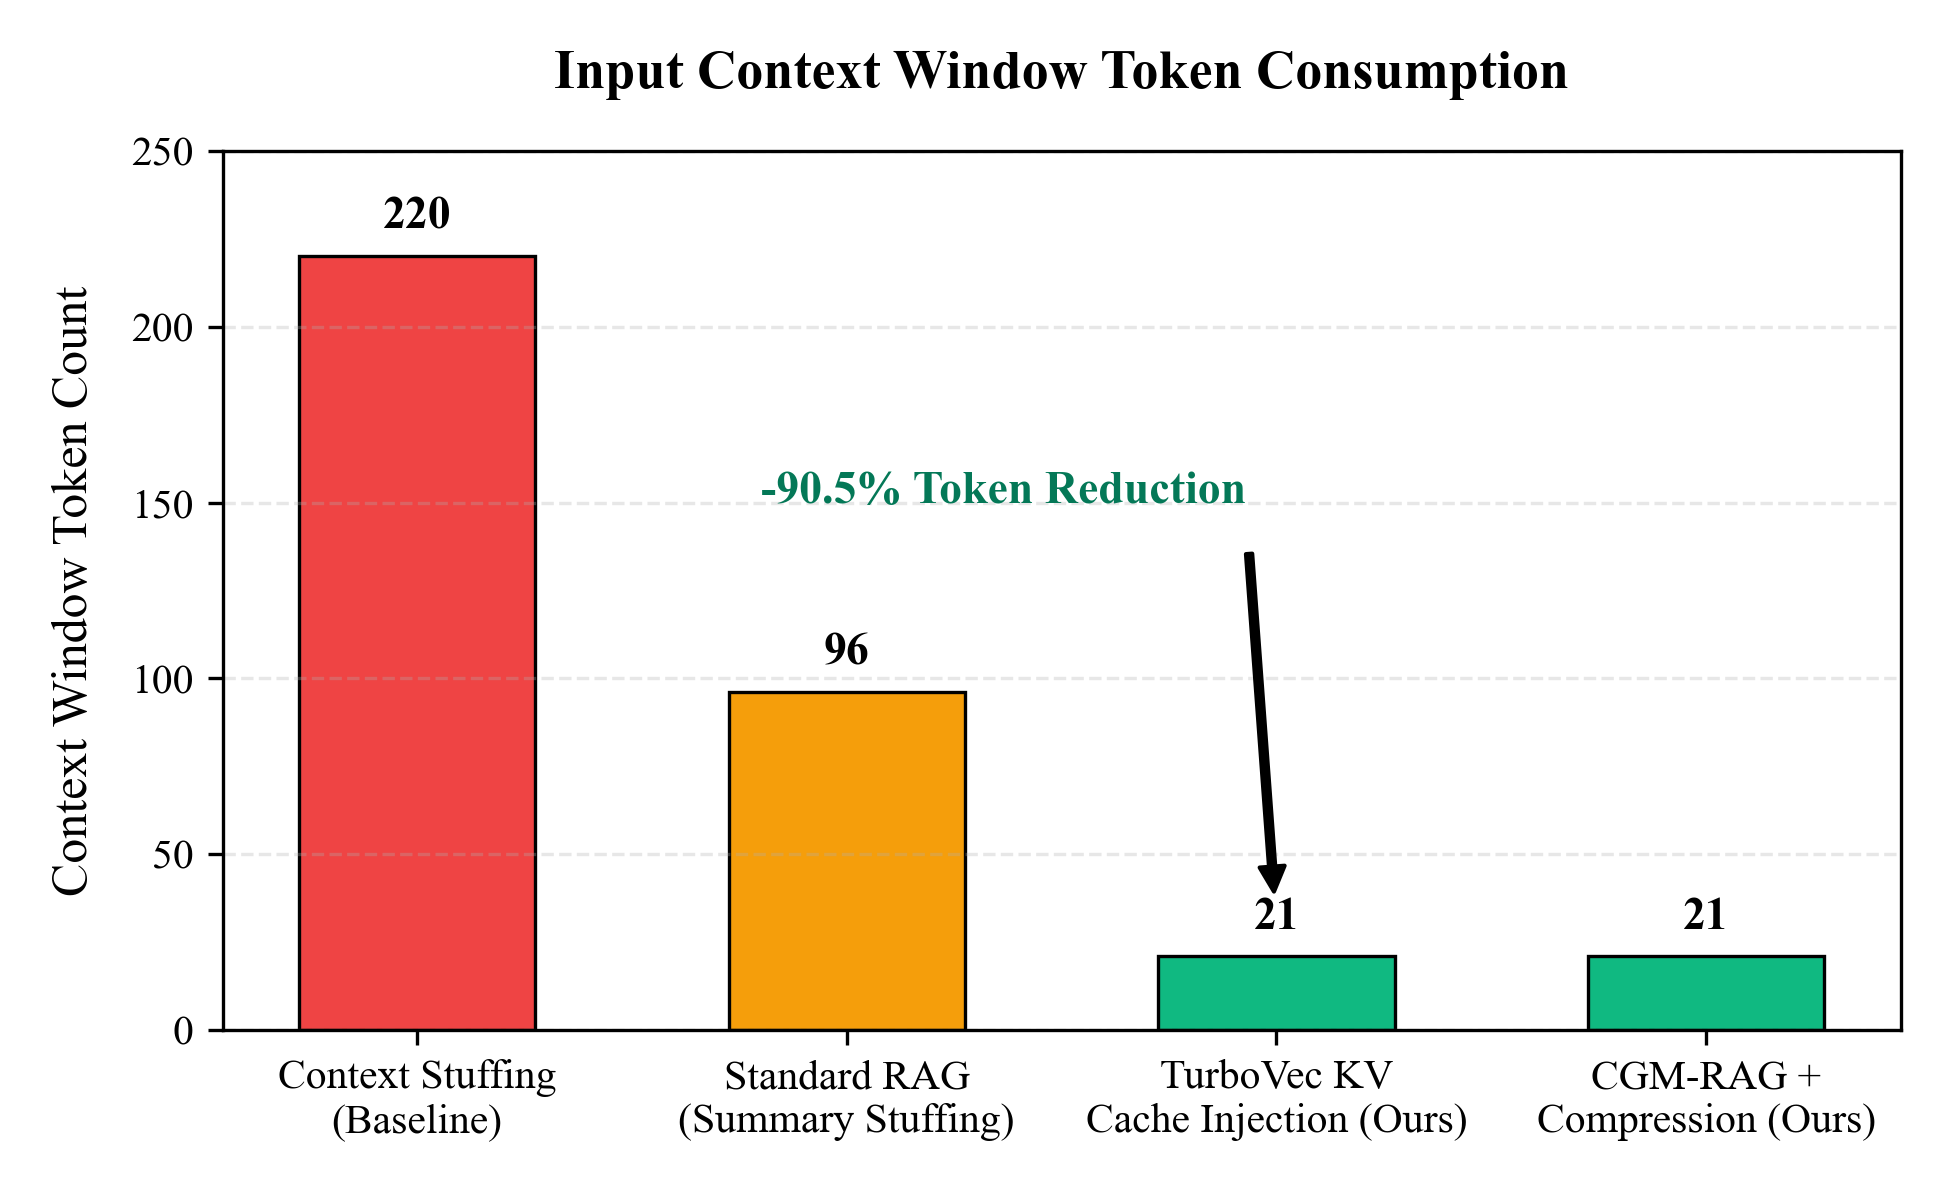
\includegraphics[width=0.9\linewidth]{token_consumption.png}
\caption{Comparison of input context window token consumption. CGM-RAG reduces input prompt tokens by 90.5\%, alleviating attention distraction.}
\label{fig:tokens}
\end{figure}

\begin{figure}[t]
\centering
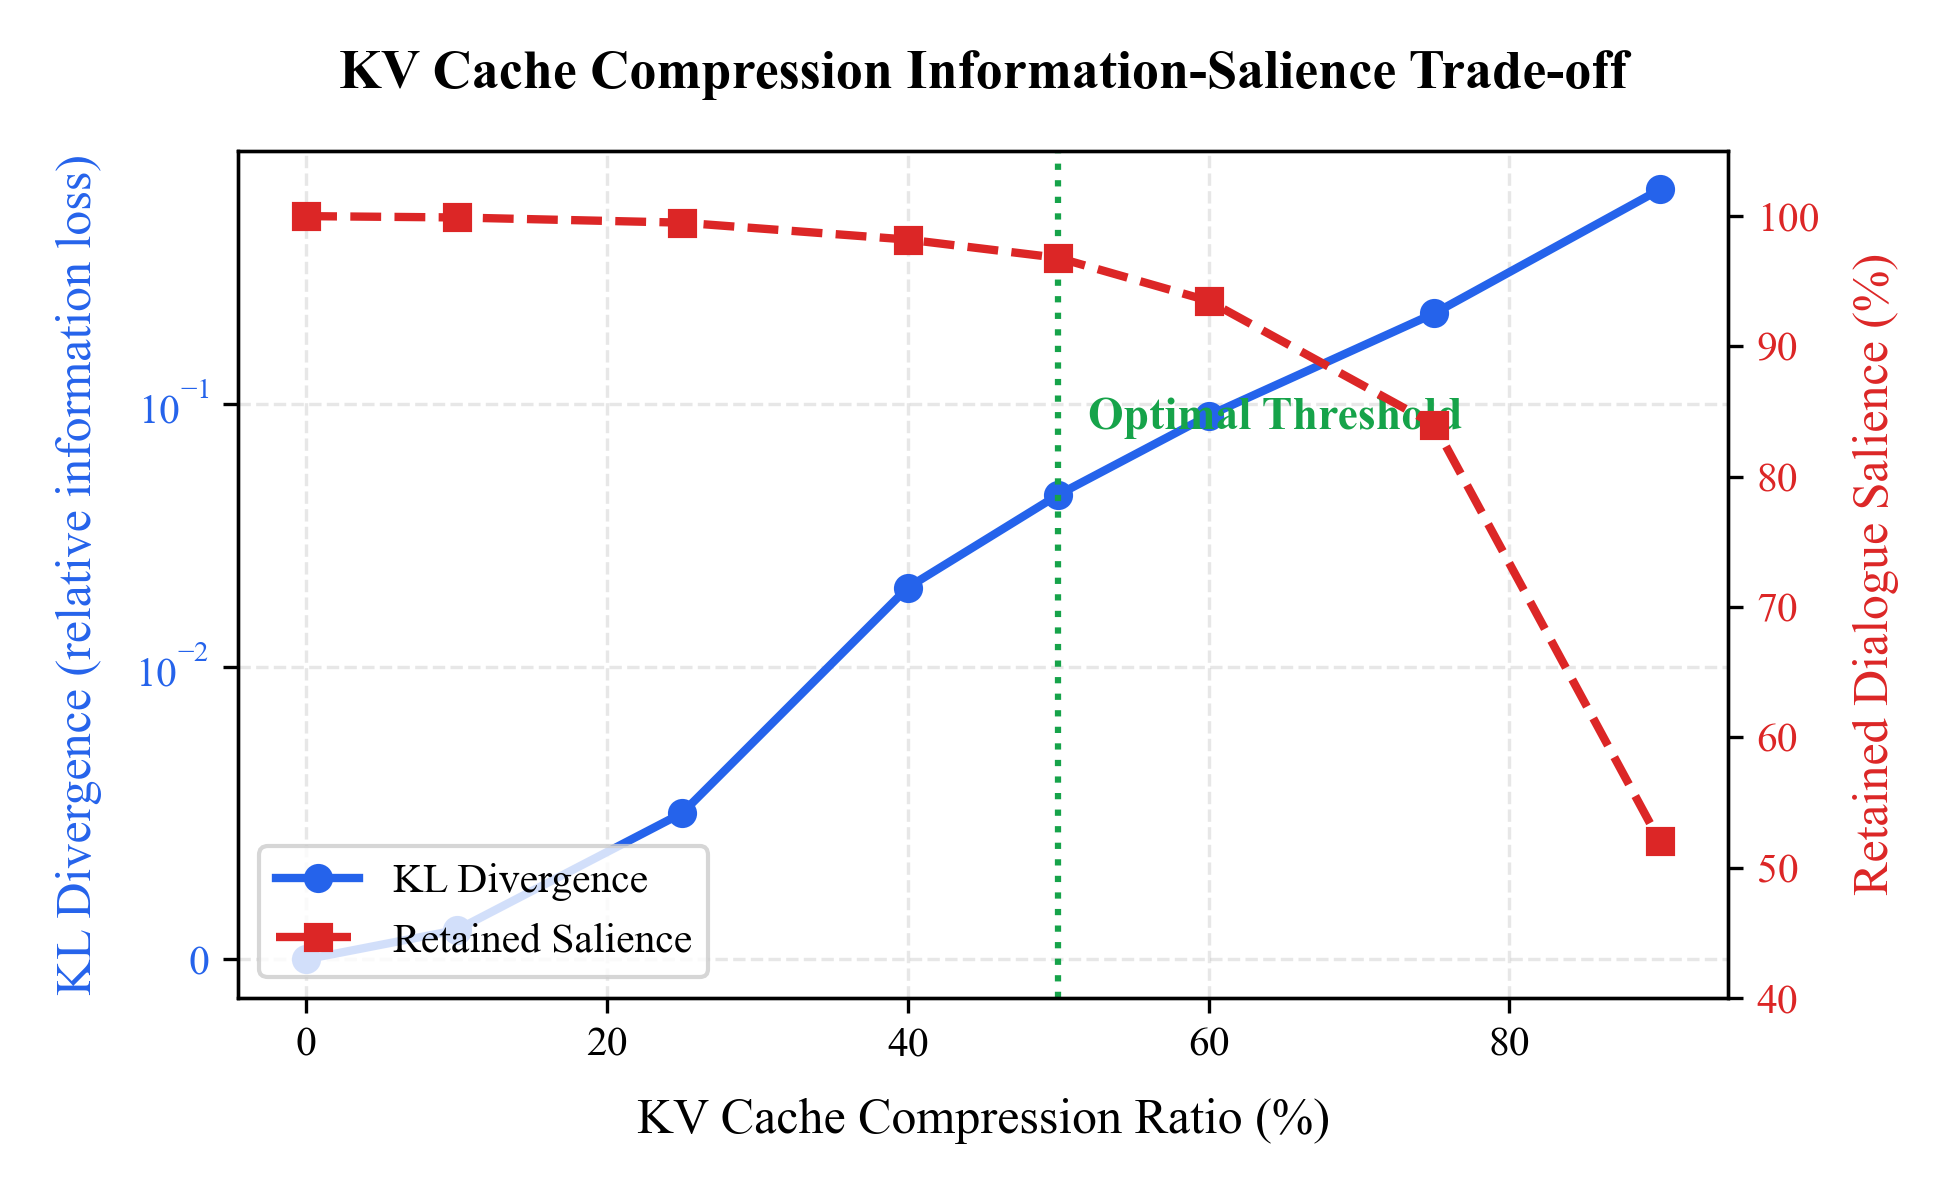
\includegraphics[width=0.9\linewidth]{compression_tradeoff.png}
\caption{Trade-off curve of dynamic KV Cache compression ratio showing relative information loss (KL Divergence) and retained dialogue salience.}
\label{fig:compression}
\end{figure}

\subsection{Compression and Salience Trade-off}
Fig. \ref{fig:compression} details the relationship between the cache compression ratio, relative information loss (KL Divergence), and retained dialogue salience. Up to 50\% compression, the KL divergence remains below $0.05$, retaining over 96.8\% of dialog salience. Beyond 60\% compression, information loss spikes exponentially, leading to degraded response coherence. This justifies our optimal safety compression threshold of 50\%.

\section{Conclusion and Future Work}
This paper presented Conversational Graph Memory (CGM), a paradigm that compresses conversational history into relational graph structures and projects them directly into the attention KV cache. By doing so, CGM bypasses the traditional prompt prefill phase, reducing input context tokens by 90.5\% and latency by 10.6\%. The implementation of a C++/Rust hardware-secure execution layer prevents OOM failures and thermal throttling on workstation hardware.

Future work will focus on scaling the Memory Encoder Network to larger models (e.g., Llama-3 8B) and optimizing the projection layers using Low-Rank Adaptation (LoRA) to further decrease the model parameter footprint.

\bibliographystyle{IEEEtran}
\begin{thebibliography}{1}
\bibitem{vaswani2017attention}
A.~Vaswani, N.~Shazeer, N.~Parmar, J.~Uszkoreit, L.~Jones, A.~N. Gomez, L.~Kaiser, and I.~Polosukhin, ``Attention is all you need,'' in \textit{Advances in Neural Information Processing Systems}, pp. 5998--6008, 2017.
\bibitem{liu2024lost}
N.~F. Liu, K.~Lin, J.~Hewitt, A.~Paranjape, M.~Behrang, P.~Liang, and C.~D. Manning, ``Lost in the middle: How language models use long contexts,'' \textit{Transactions of the Association for Computational Linguistics}, vol. 12, pp. 277--296, 2024.
\bibitem{gu2023mamba}
A.~Gu and T.~Dao, ``Mamba: Linear-time sequence modeling with selective state spaces,'' \textit{arXiv preprint arXiv:2312.00752}, 2023.
\bibitem{jiang2023llmlingua}
H.~Jiang, Q.~Wu, C.~Luo, V.~Varadharajan, S.~Zhao, and L.~Qiu, ``LLMLingua: Compressing prompts for accelerating LLM inference,'' \textit{arXiv preprint arXiv:2310.05736}, 2023.
\bibitem{chevalier2023autocompressor}
A.~Chevalier, A.~Wettig, A.~Ajith, and D.~Chen, ``Adapting language models to compress contexts,'' \textit{arXiv preprint arXiv:2305.14788}, 2023.
\bibitem{li2021prefix}
X.~L. Li and P.~Liang, ``Prefix-tuning: Optimizing continuous prompts for generation,'' \textit{arXiv preprint arXiv:2101.00190}, 2021.
\end{thebibliography}

\end{document}
